\documentclass[10pt]{beamer}

\graphicspath{{Images/}{./}}
\usepackage{booktabs,hyperref,mathabx}
%\usetheme{default}
%\usetheme{AnnArbor}
%\usetheme{Antibes}
%\usetheme{Bergen}
%\usetheme{Berkeley}
%\usetheme{Berlin}
%\usetheme{Boadilla}
%\usetheme{CambridgeUS}
%\usetheme{Copenhagen}
%\usetheme{Darmstadt}
%\usetheme{Dresden}
%\usetheme{Frankfurt}
%\usetheme{Goettingen}
%\usetheme{Hannover}
%\usetheme{Ilmenau}
%\usetheme{JuanLesPins}
%\usetheme{Luebeck}
\usetheme{Madrid}
%\usetheme{Malmoe}
%\usetheme{Marburg}
%\usetheme{Montpellier}
%\usetheme{PaloAlto}
%\usetheme{Pittsburgh}
%\usetheme{Rochester}
%\usetheme{Singapore}
%\usetheme{Szeged}
%\usetheme{Warsaw}

%----------------------------------------------------------------------------------------
%	SELECT COLOR THEME
%----------------------------------------------------------------------------------------

% Beamer comes with a number of color themes that can be applied to any layout theme to change its colors. Uncomment each of these in turn to see how they change the colors of your selected layout theme.

%\usecolortheme{albatross}
%\usecolortheme{beaver}
%\usecolortheme{beetle}
%\usecolortheme{crane}
%\usecolortheme{dolphin}
%\usecolortheme{dove}
%\usecolortheme{fly}
%\usecolortheme{lily}
%\usecolortheme{monarca}
%\usecolortheme{seagull}
%\usecolortheme{seahorse}
\usecolortheme{spruce}
%\usecolortheme{whale}
%\usecolortheme{wolverine}

%----------------------------------------------------------------------------------------
%	SELECT FONT THEME & FONTS
%----------------------------------------------------------------------------------------

% Beamer comes with several font themes to easily change the fonts used in various parts of the presentation. Review the comments beside each one to decide if you would like to use it. Note that additional options can be specified for several of these font themes, consult the beamer documentation for more information.

\usefonttheme[onlymath]{serif} % Typeset using the default sans serif font
%\usefonttheme{serif} % Typeset using the default serif font (make sure a sans font isn't being set as the default font if you use this option!)
%\usefonttheme{structurebold} % Typeset important structure text (titles, headlines, footlines, sidebar, etc) in bold
%\usefonttheme{structureitalicserif} % Typeset important structure text (titles, headlines, footlines, sidebar, etc) in italic serif
%\usefonttheme{structuresmallcapsserif} % Typeset important structure text (titles, headlines, footlines, sidebar, etc) in small caps serif

%------------------------------------------------

%\usepackage{mathptmx} % Use the Times font for serif text
%\usepackage{palatino} % Use the Palatino font for serif text

%\usepackage{helvet} % Use the Helvetica font for sans serif text
%\usepackage[default]{opensans} % Use the Open Sans font for sans serif text
\usepackage{amsfonts,amsmath,xcolor}
\usepackage[backend=biber,style=alphabetic]{biblatex}
\addbibresource{ref.bib}
%\usepackage[default]{FiraSans} % Use the Fira Sans font for sans serif text
%\usepackage[default]{lato} % Use the Lato font for sans serif text

%----------------------------------------------------------------------------------------
%	SELECT INNER THEME
%----------------------------------------------------------------------------------------

% Inner themes change the styling of internal slide elements, for example: bullet points, blocks, bibliography entries, title pages, theorems, etc. Uncomment each theme in turn to see what changes it makes to your presentation.

%\useinnertheme{default}
%\useinnertheme{circles}
%\useinnertheme{rectangles}
\useinnertheme{rounded}
%\useinnertheme{inmargin}

%----------------------------------------------------------------------------------------
%	SELECT OUTER THEME
%----------------------------------------------------------------------------------------

% Outer themes change the overall layout of slides, such as: header and footer lines, sidebars and slide titles. Uncomment each theme in turn to see what changes it makes to your presentation.

%\useoutertheme{default}
%\useoutertheme{infolines}
%\useoutertheme{miniframes}
%\useoutertheme{smoothbars}
%\useoutertheme{sidebar}
%\useoutertheme{split}
%\useoutertheme{shadow}
%\useoutertheme{tree}
%\useoutertheme{smoothtree}

%\setbeamertemplate{footline} % Uncomment this line to remove the footer line in all slides
%\setbeamertemplate{footline}[page number] % Uncomment this line to replace the footer line in all slides with a simple slide count

%\setbeamertemplate{navigation symbols}{} % Uncomment this line to remove the navigation symbols from the bottom of all slides

%----------------------------------------------------------------------------------------
%	PRESENTATION INFORMATION
%----------------------------------------------------------------------------------------

\title[Algebraic Circuits Factorization]{Factorization of Polynomials in the perspective of Algebraic Circuits} % The short title in the optional parameter appears at the bottom of every slide, the full title in the main parameter is only on the title page

% \subtitle{} % Presentation subtitle, remove this command if a subtitle isn't required

\author[Soham Chatterjee]{Soham Chatterjee} % Presenter name(s), the optional parameter can contain a shortened version to appear on the bottom of every slide, while the main parameter will appear on the title slide

\institute[CMI]{Chennai Mathematical Institute \\ \smallskip \textit{sohamchatterjee999@gmail.com}} % Your institution, the optional parameter can be used for the institution shorthand and will appear on the bottom of every slide after author names, while the required parameter is used on the title slide and can include your email address or additional information on separate lines

\date[\today]{\today} % Presentation date or conference/meeting name, the optional parameter can contain a shortened version to appear on the bottom of every slide, while the required parameter value is output to the title slide

%----------------------------------------------------------------------------------------

\begin{document}

%----------------------------------------------------------------------------------------
%	TITLE SLIDE
%----------------------------------------------------------------------------------------

\begin{frame}
	\titlepage
\end{frame}

%----------------------------------------------------------------------------------------
%	TABLE OF CONTENTS SLIDE
%----------------------------------------------------------------------------------------

% The table of contents outputs the sections and subsections that appear in your presentation, specified with the standard \section and \subsection commands. You may either display all sections and subsections on one slide with \tableofcontents, or display each section at a time on subsequent slides with \tableofcontents[pausesections]. The latter is useful if you want to step through each section and mention what you will discuss.

\begin{frame}
	\frametitle{Presentation Overview} % Slide title, remove this command for no title
	
	\tableofcontents % Output the table of contents (all sections on one slide)
	%\tableofcontents[pausesections] % Output the table of contents (break sections up across separate slides)
\end{frame}

%----------------------------------------------------------------------------------------
%	PRESENTATION BODY SLIDES
%----------------------------------------------------------------------------------------

\section{Introduction and Preliminaries of Circuits} % Sections are added in order to organize your presentation into discrete blocks, all sections and subsections are automatically output to the table of contents as an overview of the talk but NOT output in the presentation as separate slides

%------------------------------------------------

\subsection{Introduction}

\begin{frame}
	\frametitle{Introduction}
	
	\begin{itemize}
	    \item We mainly study Turing Machines and Different Classes created by considering certain parameters of Turing machines like Time, Space, Randomness, Communication, Nondeterminism etc in Complexity Theory.
     \item Another model which is often our interest is Circuits. They are basically a kind of DAG (Directed Acyclic Graph) 
     \item First interest of Computer Scientists was Boolean Circuits. Here the nodes are $\wedge$ (AND), $\vee$ (OR) gates. The edges have either $\neg$ (NOT) gate or nothing and the leaves have the variables of the boolean formula.
     \item To study them better later Computer Scientists Started Algebraic Circuits where instead of $\wedge, \vee $ we have $+,\times $ and the edges have the coefficients of from the ring we are working on and leaves have the variables
	\end{itemize}
\end{frame}

\begin{frame}
	\frametitle{Introduction}
	
	\begin{itemize}
	    
     \item To evaluate the circuit we start from the bottom at go up to the root and the root represents the final Boolean formula or circuit and polynomial
     \item Now the whole reason to study algebraic circuits is not to limit ourselves to $\mathbb{F}_2$ but any field.
     \item In general, multivariate polynomial factoring has several applications including decoding of Reed-Solomon, Reed-Muller codes \cite{reedsol}, \cite{sudreedsol}, integer factoring \cite{numsieve},primary decomposition of polynomial ideals \cite{grobnerbaspolyideL} and algebra isomorphism \cite{Kayal2006ComplexityOR},\cite{grhfactpoly}.
	\end{itemize}
\vspace*{5mm}

\begin{center}
    $\boxed{\text{ In this lecture, we will talk about fields with characteristic 0}}$
\end{center}
\end{frame}

%------------------------------------------------

\begin{frame}
	\frametitle{Introduction}
	% \framesubtitle{Bullet Points and Numbered Lists} % Optional subtitle
	
	\begin{figure}[h]
	    \centering
	    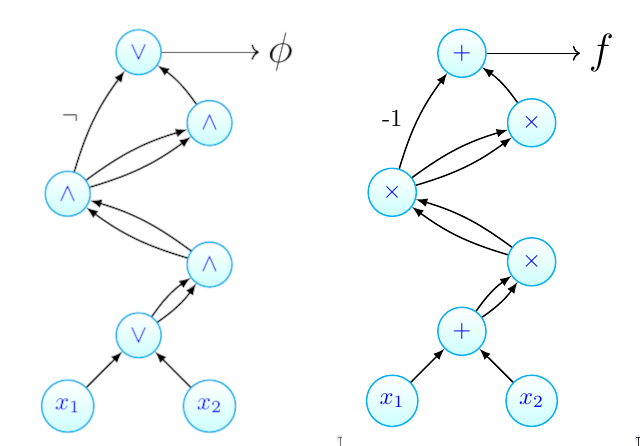
\includegraphics[width=7cm]{Images/Untitled.png}
	\end{figure}
 The left one is a Boolean circuit and the right one is an algebraic circuit or arithmetic circuit. 
 \vspace{2mm}
 
 \textbf{Note: }Some papers also have written algebraic circuits as Straight Line Program  (Just a regular day of Kaltofen and Valiant Papers)
\end{frame}

\begin{frame}
	\frametitle{Definitions}
	% \framesubtitle{Bullet Points and Numbered Lists} % Optional subtitle
	\begin{itemize}
	    \item \textbf{Size:} Size of the whole $DAG$ graph is the size of the circuit
     \item \textbf{Fan-in, Fan-out:} Fan-in = Max in degree, Fan-out = Max out-degree
     \item \textbf{ABP (Arithmetic Branching Program):} These are a special type of circuits. An algebraic branching program $(A B P)$ is a layered graph with a unique source vertex (say s) and a unique sink vertex (say $t$ ). All edges are from layer $i$ to $i+1$ and each edge is labeled by a linear polynomial. The polynomial computed by the $A B P$ is defined as $$f=\sum\limits_{\gamma: s \rightsquigarrow t}\ wt (\gamma)$$, where for every path $\gamma$ from s to $t$, the weight wt $(\gamma)$ is defined as the product of the labels over the edges forming $\gamma$.
     
     Width is the maximum number of vertices in a layer.
     \item \textbf{Formula: }Formula is an algebraic circuit with fan-out 1. (So you can not store any computation)
	\end{itemize}
\end{frame}
%------------------------------------------------


% \begin{frame}
% 	\frametitle{Blocks of Highlighted Text}
	
% 	\begin{block}{Block Title}
% 		Lorem ipsum dolor sit amet, consectetur adipiscing elit. Integer lectus nisl, ultricies in feugiat rutrum, porttitor sit amet augue.
% 	\end{block}
	
% 	\begin{exampleblock}{Example Block Title}
% 		Aliquam ut tortor mauris. Sed volutpat ante purus, quis accumsan.
% 	\end{exampleblock}
	
% 	\begin{alertblock}{Alert Block Title}
% 		Pellentesque sed tellus purus. Class aptent taciti sociosqu ad litora torquent per conubia nostra, per inceptos himenaeos.
% 	\end{alertblock}
	
% 	\begin{block}{} % Block without title
% 		Suspendisse tincidunt sagittis gravida. Curabitur condimentum, enim sed venenatis rutrum, ipsum neque consectetur orci.
% 	\end{block}
% \end{frame}

%------------------------------------------------

\subsection{Algebraic Circuit Classes}

\begin{frame}
	\frametitle{Algebraic Circuit Classes}
	\framesubtitle{$VNP$, $VP$, $VBP$, $VF$} % Optional subtitle
 From now on $n$ denotes the number of variables
	\begin{itemize}
	    \item \textbf{VP:} The class $VP$ contains all the algebraic circuits of the polynomials which has degree $poly(n)$ and size $poly(n)$. $P$ analog of algebraic circuits 
     \item \textbf{VBP:} The class $VBP$ contains all the $ABP$'s which has degree $poly(n)$ and size $poly(n)$
     \item \textbf{VF:} The class $VF$ contains all the formulas of the polynomials which has degree $poly(n)$ and size $poly(n)$
     \item \textbf{VNP:} A family of polynomials $\left\{f_n\right\}_n$ over $\mathbb{F}$ is in $VNP$ if there exist polynomials $t(n), s(n)$ and a family $\left\{g_n\right\}_n$ in VP such that for every $n$, $$f_n(\bar{x})=\sum_{w \in\{0,1\}^{t(n)}} g_n\left(\bar{x}, w_1, \ldots, w_{t(n)}\right)$$ Here, witness size is $t(n)$ and versifier circuit $g_n$ has size $s(n)$. Its basically $NP$ analogue of algebraic circuits so $VP$ with non-determinism
	\end{itemize}
	
\end{frame}

%------------------------------------------------

\subsection{Results on Classes}


\begin{frame}
\frametitle{Some results on these classes}
	\begin{itemize}
 \item $VF\subseteq VBP \subseteq VP \subseteq VNP$
 \item Any circuit of size $s$ and depth $d$ can be converted to a formula of size $s^d$ 
	    \item $VP$ is contained in $VNP$ and it is believed that this containment is strict (Valiant's Hypothesis \cite{Valiant1979CompletenessCI}).
     \item $VP= VNP\implies \#P=FP\implies P= NP$
     \item $DET$ is $VBP-complete$ \cite{Mahajan1997ACA}
     \item $PERM$ is $VNP-complete$ \cite{completeburg}
     \item There are other structural results that are well written in \cite{ramsurvey} and \cite{shpilkasurvey}
     \end{itemize}
\end{frame}

%------------------------------------------------

\section{Mathematics}
\subsection{Newton Iteration}

\begin{frame}
	\frametitle{Mathematics}
 \framesubtitle{Newton Iteration}
	
 \begin{itemize}
     \item Since we work on polynomials and  power series we assume the function is differentiable
     \end{itemize} 
 
	\begin{theorem}[Newton Iteration {\cite[Theorem 2.31]{burgalgcomp}}, \cite{gathenalgebra},\cite{Gathen1984HenselAN}]
		If $f$ is a function on any number of variables, let $(\overline{x},y)$, has a root at $g$ wrt $y$ i.e. $f(\overline{x},g(\overline{x}))=0$ then $$y_{i+1}=y_i-\left.\frac{f}{\partial_yf}\right|_{y=y_i} $$ where $y_i\equiv g\text{ mod } \langle \overline{x}\rangle^{i}$ so that $$y_{i+1}\equiv g\text{ mod }\langle \overline{x}\rangle^{i+1}$$
	\end{theorem}

 \begin{itemize}
     \item This extra variable $y$ comes because we actually shift the variables randomly by adding another variable so that the polynomial does not become zero $\overline{x}\mapsto \overline{x}+\overline{a}y+\overline{b}$  by Schwarz - Zippel Lemma \cite{schwarzippel}
          \end{itemize} 
\end{frame}

%------------------------------------------------

\subsection{Hensel Lifting}

\begin{frame}
	\frametitle{Mathematics}
 \framesubtitle{Hensel Lifting}
	\textbf{Lifting} {\cite[Section 4.1]{abpfactor}}]: Let $\mathcal{R}$ be a ring and $\mathcal{I} \subseteq \mathcal{R}$ be an ideal. Let $f, g, h, a, b \in R$ such that $f \equiv g h(\bmod \mathcal{I})$ and $a g+b h \equiv 1(\bmod \mathcal{I})$. Then we call $g^{\prime}, h^{\prime} \in \mathcal{R}$ a lift of $g, h$, if
	    \begin{enumerate}
\item $f \equiv g^{\prime} h^{\prime}\left(\bmod \mathcal{I}^2\right)$
\item ${g}^{\prime} \equiv  {g}(\bmod \mathcal{I})$ and $h^{\prime} \equiv h(\bmod \mathcal{I})$, and
\item $\exists\ a^{\prime}, b^{\prime} \in \mathcal{R} \quad a^{\prime} g^{\prime}+ {b}^{\prime} h^{\prime} \equiv 1\left(\bmod \mathcal{I}^2\right)$.
\end{enumerate}

 \begin{theorem}[Hensel Lifting {\cite[Section 4.1]{abpfactor}},\cite{gathenalgebra},\cite{Gathen1984HenselAN}]
		Let $\mathcal{R}$ be a ring and $\mathcal{I} \subseteq \mathcal{R}$ be an ideal. Let $f, g, h, a, b \in R$ such that $f \equiv h\pmod{\mathcal{I}}$ and ${ag}+{bh} \equiv 1(\bmod \mathcal{I})$. Then we have there exists a lift ${g}^{\prime}, h^{\prime}$ of $g, h$ and for any other lift ${g}^*, h^*$ of ${g}, {h}$, $\exists$ ${u} \in \mathcal{I}$ such that $$g*\equiv g^{\prime}(1+u) \pmod  {\mathcal{I}^2} \text{ and } h* \equiv h^{\prime}(1-u) \pmod {\mathcal{I}^2}$$
\end{theorem}

\end{frame}

%------------------------------------------------
\section{Uni-variate Polynomial Factorization}
\subsection{Field with finite characteristic (prime)}
\begin{frame}[allowframebreaks]
\frametitle{Uni-variate Polynomial Factorization}
\framesubtitle{Field with finite characteristic (prime)}
\begin{itemize}
	\item We are in the field $\mathbb{F}_q$, $q=p^n$ $char(\mathbb{F}_q)=p$. Input $f$ with $\deg f=d$
\end{itemize}
{\textbf{Preprocess:}}
\begin{itemize}
	\item \textbf{Square-free} Take $gcd(f,\partial f)$ to get a square free factor. Call this $f$
	\item \textbf{Distinct-degree} From 1 to $\frac{d}{2}$ we take the $gcd(f,x^{q^i}-x)$ to output the product of all $i-$degree factors of $f$. $f=\prod\limits_{i\in [k]}f_i$ each $f_i$ irreducible and $\deg f_i=\frac{d}{k}$
\end{itemize}
	
	\begin{theorem}[{\cite[Theorem 14.2]{gathenalgebra}}]
		For any $d\geq 1$, $x^{q^d}-x\in \mathbb{F}_q[x]$ is the product of all monic irreducible polynomials in $\mathbb{F}_q[x] $ whose degree divides $d$
	\end{theorem}
	\begin{itemize}
		\item This also gives an algorithm to check if the polynomial is reducible.
		\item If $f,g$ are co-prime polynomials in any field $\mathbb{F}$ then $\mathbb{F}[x]/\langle fg\rangle\cong \mathbb{F}[x]/\langle f\rangle\times \mathbb{F}[x]/\langle g\rangle$
	\end{itemize}
	\vspace*{5mm}
	
	{\large{Barlekamp Algorithm:}}({\cite{barlelargefield},\cite[Section 14.8]{gathenalgebra}},{\cite[Section 4.6.2]{knuthvol2}},\cite{ramalgcomp2017})
	\begin{itemize}
		\item Factoring $f$ is factoring $\mathcal{A}:=\bigtimes\limits_{i=1}^k \underbrace{\mathbb{F}_q[x]/\langle f_i\rangle}_{=\mathbb{F}_{q'}}$
		\item Want to find the Isomorphism. We know the $RHS$
		\item Any $g\in \mathcal{A}$ is a $k-$tuple $(a_1,a_2,\dots,a_k)$, $a_i\in \mathbb{F}_q[x]/\langle f_i\rangle\implies g\equiv a_i\pmod {f_i}$. If $a_i\in \mathbb{F}_p$ then $g^p\equiv g$ in $\mathcal{A}$
		\item Such $g$ gives a factor of $f$ as $g^p-g\equiv 0 \ \text{mod }f\implies \prod\limits_{\alpha\in \mathbb{F}_p}(g-\alpha)\equiv 0\ \text{mod }f	\implies \left. \prod_{i\in [k]}f_i\right| \prod\limits_{\alpha\in \mathbb{F}_p}(g-\alpha)$
		\item $\left\{ g\in \mathbb{F}_q[x]\mid g^p\equiv g\pmod f \right\}$ is a vector space over $\mathbb{F}_p$. So we do some system of linear equation solving
		\item \textbf{Time Complexity:} $\tilde{O}(p(dn)^{\omega})$ where $\omega$ the Matrix Multiplication Exponent
	\end{itemize}
	
	Barlekamp Algorithm is the oldest polynomial factorization algorithm. Later there are much improvements in the complexity of factorization with the addition  of randomization.
	\begin{theorem}
		$\alpha\in \mathbb{F}_p*$ is  a square or quadratic residue $\iff \alpha^{\frac{p-1}{2}}\equiv 1\pmod p$
	\end{theorem}
	\begin{itemize}
		\item $Pr_{\alpha\in_R \mathbb{F}_p\asterisk}[\alpha \text{is a quadratic residue}]=\frac12$
	\end{itemize}
	\vspace*{3mm}
	
	{\large{Cantor-Zassenhaus Algorithm}}(\cite[Section 14.3]{gathenalgebra},\cite{ramalgcomp2017},\cite{Zassenhaus1969OnHF})
	\begin{itemize}
		\item WLOG we assume $p>2$
		\item $a\in_R\mathbb{F}_p$. $g=f(x-a)$, the roots if $g$ have different quadratic residuocity.
		\item Pick $\alpha\in_R\mathbb{F}_p$. If $\alpha+a$ is a zero of $f(x-a)$ and it is a square then it also a root of $gcd(f(x-a),x^{\frac{p-1}{2}}-1)$
		\item So we output $gcd(f(x),(x+a)^{\frac{p-1}{2}}-1)$
		\item \textbf{Time Complexity:} $\tilde{O}(d^{\omega}\log q)$
	\end{itemize}
\end{frame}

%------------------------------------------------

\subsection{Field with characteristic 0}
\begin{frame}[allowframebreaks]
\frametitle{Uni-variate Polynomial Factorization}
\framesubtitle{Field with characteristic 0}
\begin{itemize}
	\item We will talk about polynomial factorization in $\mathbb{Q}[x]$ or $\mathbb{Z}[x]$
	\item Coefficients of $f$ are less than $2^{l-1}$
	\item We will talk about the algorithm discovered by Lenstra, Lenstra, Lovasz in 1982 \cite{lllalgo} using shortest vectors.
	\item $\|f\|_{\infty}=A$
\end{itemize}
\begin{theorem}[Mignotte's Bound \cite{Mignotte1974AnIA}]
	Any root $\alpha\in\mathbb{C}$ of a polynomial $f(x)=\sum\limits_{i=0}^na_ix^i\in \mathbb{Z}[x]$ satisfies $\alpha\leq n\max \{|a_i\}$
\end{theorem}
\begin{theorem}
	Any factor $g$ of $f$ has coefficient of magnitude at most $2^{(l+\log n-1)n}$
\end{theorem}
\begin{theorem}[{\cite[Lemma 16.20]{gathenalgebra}}]
	Let $f,g\in \mathbb{Z}[x]$ have positive degrees $n,k$ respectively and suppose that $u\in\mathbb{Z}[x]$ is non-constant, monic, and divides both $f,g$ modulo $m$ for some $m\in \mathbb{N}$ with $\|f\|^k\|g\|^n<m$. Then $gcd(f,g)\in \mathbb{Z}[x]$
\end{theorem}

{\large{$L^3$ Algorithm}}(\cite{lllalgo},{\cite[Chapter 16]{gathenalgebra}})
\begin{itemize}
	\item Assume that $f$ is square free. Find the smallest prime $p$ such that $p\nmid a_n$ and $f\pmod p$ is square free
	\item Using Barlekamp algorithm compute a factorization of $f\equiv f_0g_0\pmod p$ where $g_0\pmod p$ is monic irreducible and co-prime to $h_0$
	\item Compute $f\equiv g_kh_k\pmod {p^{2^k}}$ by Hensel Lifting for $k=\lceil \log 2n^3l\rceil$
	\item Find $(\tilde{g},l_k)$ such that $\tilde{g}\equiv g_kl_k\pmod{p^{2^k}}$ with $\deg \tilde{g}<n$. Coefficients of $\tilde{g}$ have bit-size $\leq n(l+\log n)$
	\item Output $gcd(f,\tilde{g})$
	\item \textbf{Time Complexity: }$\tilde{O}(n^{10}+n^8\log^2A)$ 
\end{itemize}

In 4-th Step this requires a small root of a linear system. Which involves short vector in a lattice system.  But Shortest Vector Problem is NP-Hard \cite{svpnph}, even constant approximation of it is also $NP-hard$ \cite{svpconstap}. But we need $2^n-$approximation so it is doable.

\end{frame}

%------------------------------------------------
\section{Multi-variate Polynomial Factorization}

\begin{frame}
	\frametitle{Multi-variate Polynomial Factorization}
\begin{itemize}
	\item Since we can do uni-variate factorization quite easily and in polynomial time in most of the multivariate factorization we first some how make the polynomial  uni-variate  then factorize there and bring it back to multivariate with some sort of lifting.
	\item Most of the algorithms mainly first apply a random shift to the variables first. 
	\item In case of multivariate factoring we see if we can say anything about the closure of the algebraic complexity classes.
	\item There are surveys for polynomial factorization \cite{kalsurvey},\cite{Kaltofen2020PolynomialF1},\cite{forbessurvey} to get much more depth
\end{itemize}
\end{frame}

%------------------------------------------------

\subsection{Low Degree Polynomial factorization}
\begin{frame}
	\frametitle{Low Degree Polynomial factorization}
	
\begin{itemize}
    \item By low degree we mean individual degrees are bounded by some constant
\end{itemize}

\vspace{5mm}
 
\begin{theorem}[\cite{lowdegfact}]
    Let $P\in\mathbb{F}[\overline{x}]\setminus\{0\}$ be such that $ \deg_{x_i}P\leq r$ for $i\in[n]$ and $f $ is a factor of P where $char(\mathbb{F})=0$. If there exists a formula (circuit) of size $s$ and depth $\Delta$ computing $P$ then there exists a formula (circuit) of depth $\Delta+5$ and size $poly((nr)^r,s)$ that computes $f$
\end{theorem}
\vspace{5mm}

\begin{itemize}
    \item It calculates from $0$ to $d$ calculates the Homogeneous part of $P$ 
    \item Then it uses Newton's Iteration to calculate the next degree Homogeneous Part
\end{itemize}
\end{frame}
%------------------------------------------------

\subsection{VP closed under factorization}
\begin{frame}
	\frametitle{$VP$ closed under factorization}
	\begin{theorem}[\cite{chou2019closure},\cite{Kaltofen1989FactorizationOP}]
	Let $f\in\mathbb{F}[x_1, x_2,\dots, x_{n-1}, y]$ be an $n$-variate degree $d$ polynomial which can be computed by an arithmetic circuit of size at most $s$. If $g$ and $h$ are polynomials of degree at least 1 such
	that $f = g  h$ and $gcd(g, h) = 1$, then $g$ and $h$ have a circuit of size at most $poly(s, n, d)$.
	\end{theorem}
	
	\begin{theorem}[\cite{chou2019closure},\cite{kalhensel}]
Let $f \in \mathbb{F}\left[x_1, x_2, \ldots, x_{n-1}, y\right]$ be an $n$-variate degree $d$ polynomial which can be computed by an arithmetic circuit of size at most s. If there is a polynomial $g$ and an integer e such that $f=g^e$, then $g$ has a circuit of size at most ${poly}(s, n, d)$.
	\end{theorem}
	
	
\end{frame}

%------------------------------------------------

\subsection{VBP closed under factorization}
\begin{frame}
	\frametitle{$VBP$ closed under factorization}
	
	\begin{theorem}[\cite{abpfactor}]
		Let $p$ be a polynomial over a field $F$ with characteristic 0. For all factors $q$ of $p$, we have $$size_{ABP} (q) \leq poly(size_{ABP} (p))$$
	\end{theorem}
	\vspace{5mm}
 
	\begin{itemize}
	    \item We preprocess by random shift and introduce new variable $z$ to track total degree for $\overline{x}$ and bring multiplicity of one irreducible factor to 1 to get $\hat{p}(\overline{x},y,z)$
     \item Factor $\hat{p}(\overline{x},y,0)$ to have $\hat{q}(\overline{x},y)$ then Hensel Lift
     \item At the end we do some solving linear equations to get the exact $q$
	\end{itemize}
\end{frame}

%------------------------------------------------

\subsection{More Factorization Results}
\begin{frame}[allowframebreaks]
	\frametitle{More Factorization Results}
 \begin{itemize}
     \item These are true for exponential degree circuits also.
 \end{itemize}
 
	\begin{theorem}[{\cite[Theorm 1]{dutta2017discovering}}]
	    If $f=u_0u_1$ is a nonzero product in the polynomial ring $\mathbb{F}[\overline{X}]$ with $size(f)+size(u_0)\leq s$ then every factor  of $u_1$ has a circuit of size $poly(s+\deg(sqfree(u_1)))$
	\end{theorem}
 
	\begin{theorem}[{\cite[Theorem 3]{dutta2017discovering}}]
		The classes $V F\left(n^{\log n}\right), V B P\left(n^{\log n}\right), V N P\left(n^{\log n}\right)$ are all closed under factoring.
  
Moreover, there exists a randomized poly $\left(n^{\log n}\right)$-time algorithm that: for a given $n^{O(\log n)}$ sized formula (resp. ABP) $f$ of poly(n)-degree, outputs $n^{O(\log n)}$ sized formula (resp. ABP) of a nontrivial factor of $f$ (if one exists).
	\end{theorem}
	\framebreak
 
	\begin{itemize}
	    \item In both theorems we random shift and get $\hat{f}(\overline{x},y)$ and think as if we are in the ring $\mathbb{F}[[\overline{x}]][y]$ 
     \item $\hat{f}$ splits in this ring and then we approximate till $\deg \hat{f}$
     \item Now we factor $\hat{f}(\overline{0},y)=\hat{f}\pmod {\langle \overline{x}\rangle}$. Then Newton's Iteration to approximate 
     \item In the end we again do some solving of the system of linear equations to get the final factor of $f$ 
     \item Then we multiply some factors to get a factor of $u_1$ where we use a trick of Kaltofen
	\end{itemize}
 \begin{theorem}[{\cite[Theorem 14]{dutta2017discovering}}]
     The approximative classes $\overline{V F}\left(n^{\log n}\right), \overline{V B P}\left(n^{\log n}\right), \overline{V N P}\left(n^{\log n}\right)$ are all closed under factoring.
 \end{theorem}
\end{frame}

%------------------------------------------------

\section{Black-Box Factorization}
\begin{frame}[allowframebreaks]
	\frametitle{Black-Box Multi-variate Polynomial Factorization}
	
	\begin{theorem}[Hilbert Irreducibility Theorem \cite{KALTOFEN1985123},\cite{ramalgcomp2017},\cite{KALblackbox}]
		Let $f\left(x, y_1, \ldots, y_n\right)$ be a degree $d$ polynomial which is monic in $x$. Suppose $S \subseteq \mathbb{F}$ and ${Pr}_{\bar{a}, \bar{b} \in S^n}\left[f\left(x, a_1 t+b_1, \ldots, a_n t+b_n\right) \text { is reducible }\right] \geq \frac{O\left(d^5\right)}{|S|}$ then $f\left(x, y_1, \ldots, y_n\right)$ is reducible.
	\end{theorem}
	
	\begin{itemize}
		\item  Hilbert’s irreducibility theorem, which in one formulation says that restricting an irreducible polynomial to a random two-dimensional subspace keeps the polynomial irreducible with high probability. 
		\item They restrict a polynomial $f$ to a random two-dimensional subspace does not change the number of irreducible factors of $f$ . 
		\item Given this, multivariate factoring algorithms proceed as follows. First, restrict the polynomial to a randomly chosen two-dimensional space. 
		\item Then, perform bi-variate factorization of the restricted polynomial. Finally, lift each factor to the whole space.
	\end{itemize}
	
	\begin{theorem}[\cite{KALblackbox}]
	    The Black Box Polynomial Factorization algorithm can  output a factor in polynomially many arithmetic steps as a function of $n$ and $\deg(f)=d$ with the right answer probability at least $\frac{O(d^6)}{|S|}$ 
	\end{theorem}
\end{frame}

\section{Open Questions}
\begin{frame}{Open Questions}
    \begin{enumerate}
    	\item Randomized uni-variate algorithm in $\tilde{O}(d\log^2 q)$
        \item $VF$ or $\overline{VF}$ is closed under factors
        \item Factor closure is also not known for other models like ROABP (Read-once Oblivious ABP), Constant depth circuits
        \item We also don't know any algorithm to find the poly size ABP factor. We have existential proof in \cite{abpfactor}
        \item If we have the circuit of $f=g^p$ with size $s$ where $g$ is irreducible in $\mathbb{F}_p[\overline{x}]$ there is a circuit of $g$ in $poly(s,n)$
        \item  If we have a circuit of $f$ with size $s$ and $\deg f=d$, $f=gh$ where $\deg g =\delta$ then there is a randomized algorithm to find a circuit of $g$ with size $poly(s,n,\delta)$ [Factor Conjecture]
    \end{enumerate}
\end{frame}

%------------------------------------------------
\begin{frame}[allowframebreaks] % Use [allowframebreaks] to allow automatic splitting across slides if the content is too long
	\frametitle{References}
	
% 	\begin{thebibliography}{99} % Beamer does not support BibTeX so references must be inserted manually as below, you may need to use multiple columns and/or reduce the font size further if you have many references
% 		\footnotesize % Reduce the font size in the bibliography
		
% 		\bibitem[Leslie G. Valiant, 1979]{val79}
% 			Leslie G. Valiant, 1979
% 			\newblock Completeness classes in algebra
% 			\newblock \emph{In Proceedings of the 11h Annual
% ACM Symposium on Theory of Computing, April 30 - May 2, 1979, Atlanta, Georgia,
% USA, pages 249–261, 1979}
			
% 		\bibitem[Kennedy, 2023]{p2}
% 			Annabelle Kennedy (2023)
% 			\newblock Publication title
% 			\newblock \emph{Journal Name} 12(3), 45 -- 678.
% 	\end{thebibliography}

\printbibliography
\end{frame}


%----------------------------------------------------------------------------------------
%	CLOSING SLIDE
%----------------------------------------------------------------------------------------

\begin{frame}[allowframebreaks] % The optional argument 'plain' hides the headline and footline
	\begin{center}
		{\Huge The End}
		
		\bigskip\bigskip % Vertical whitespace
		
		{\LARGE Questions? Comments? Suggestions?}
	\end{center}
\end{frame}

%----------------------------------------------------------------------------------------

\end{document} 